%************************************************
\chapter{Discussion}
\label{chp:Discussion}
%************************************************
%\section{Parallel processing streams and their functional significance}
%Parallel processing seems to be a successful evolutionary strategy conserved throughout phyla. Other than the visual system, the olfactory system of the nematode C elegans \parencite{Chalasani2007} and the auditory cortex of mammals \parencite{Scholl2010} are some examples where parallel circuits compute ON and OFF signals separately. 
\section{Neural correlates implementing direction selectivity in the ON and the OFF pathways}
We found that elementary motion-sensitive neurons T4 and T5 in \textit{Drosophila} regardless of their directional tuning and contrast preferences for ON or OFF stimuli implement a preferred direction enhancement on the preferred side of their receptive field and a null direction suppression on the null side. The presynaptic cells for T4 cells are Mi1, Tm3, TmY15, Mi4, Mi9, C3, and CT1. The presynaptic cells for T5 cells are Tm1, Tm2, Tm4, TmY15, Tm9, CT1, LT33, and Tm23. Moreover, each subtype of a T4 cell receives synaptic input from another T4 cell of the same type. For T5 cells, the same applies. 

Blocking Mi1 completely abolished responses to ON edges, and blocking Tm3 mostly affected responses at high speeds \parencite{Ammer2015}. Therefore, Tm3 seems to be specifically needed to detect the direction of ON edges at high velocities. Mi1 provides excitatory cholinergic inputs to the central part of T4 dendrites. Mi9 provides inhibitory glutamatergic inputs to the preferred side of T4 dendrites. The preferred direction enhancement or the multiplication-like nonlinearity arises from the coincidence of cholinergic excitation and release from glutamatergic inhibition \parencite{Groschner2022}. This 'multiplicative disinhibition' represents the opposite of divisive inhibition. GABAergic inhibitory inputs on the null sides Mi4, C3, and CT1 provide the divisive inhibition or the null direction suppression. Why are there multiple cells providing input on the null side and the specific contributions of each of these cells on the null side remain to be investigated.

In the OFF pathway, selectively blocking individual Tm cells or combinations of them resulted in a range of effects on gratings and edge responses. However, no specific stimulus space could be identified where the contributions of different cells could be segregated \parencite{Serbe2016}. Tm1, Tm2, Tm4, and Tm9 provide excitatory cholinergic inputs on T5 dendrites. How is preferred direction enhancement implemented in T5 cells, with a cholinergic input on the preferred side? CT1 is the only GABAergic input providing inhibition on the null side of T5 dendrites. Does CT1 provide null direction suppression to the T5 dendrites? Why are there 3 cells providing inhibitory input on the null side of T4 dendrites compared to 1 cell providing inhibitory input on the null side of T5 dendrites? These questions are still being investigated in the OFF pathway. 

\section{Effect of voltage to calcium transformation on T4 output signals}
%In addition to the dendritic integration of postsynaptic voltages or after the action potential is generated, further computations can occur in the transformation between voltage and calcium, or between calcium and neurotransmitter release. Neuronal signaling and information processing involves the transformation of membrane voltage into calcium signals, which lead to transmitter release. 
%In our second manuscript \ref{sct:manuscript_mishra_haag}, 
We showed that the voltage to calcium transformation in T4c neurons enhances their direction selectivity. The calcium signals in T4c cells had a significantly higher direction selectivity and tuning compared to the membrane voltage across different stimuli conditions. The direction selectivity index for calcium signals compared with voltage signals for a few stimuli conditions was previously found to be higher in a study in T5 cells using ASAP2f as an optical voltage indicator \parencite{Wienecke2018}. How does this affect the output signal of T4/T5 neurons?

As calcium is required for neurotransmitter release, this is expected to increase the direction selectivity of T4/T5 cells' output signals. In the lobula plate, the T4/T5 cells provide inputs onto large lobula plate tangential cells that are depolarized during preferred and hyperpolarized during null direction motion \parencite{Mauss2014}. For example, the vertical system (VS) cells with dendrites in layer 4 receive direct excitatory inputs from downward tuned T4d/T5d neurons causing depolarization during motion in the downward preferred direction. These VS cells also receive indirect inhibitory inputs from upward tuned T4c/T5c neurons via the glutamatergic LPi3-4 neurons projecting from layer 3 to layer 4 causing hyperpolarization in VS cells during motion in the upward null direction. Upon silencing the LPi3-4 neurons’ synaptic output via tetanus toxin, the VS neurons' depolarization response in the preferred direction did not change, but the null direction response was absent \parencite{Mauss2015}. This suggests T4/T5 do not release any transmitter in response to the null direction motion, which matches our findings for the calcium responses. Thus, the voltage to calcium transformation increases direction selectivity in T4/T5 cells and this enhances direction selectivity in the downstream neurons. 

\section{Differential expression of voltage-gated calcium channels}

In manuscript \ref{sct:manuscript_mishra_haag}, we built a model to capture the voltage to calcium transformation in T4c, Mi1, and Tm3 cells. A simple model with a single low-pass filter was able to reproduce the calcium responses in non-direction-selective Mi1 and Tm3 cells, whereas a more complex model combining the output of two low-pass filters via a multiplication was required to reproduce T4c calcium responses. The direction selectivity for the simple model signals for T4c was lower compared to the multiplicative model. This suggests that voltage-calcium transformation in Mi1 and Tm3 cells is different from those in T4c cells. 

Differential expression of voltage-gated calcium channels in these cells could explain the different voltage to calcium transformation. The voltage-gated calcium channels mediate depolarization-induced calcium influx that drives the release of neurotransmitters. The $\alpha1$-subunit of the voltage-gated calcium channels form the ion-conducting pore, which makes it distinct from other calcium channels. Three families of genes encode $\alpha1$ subunits. \textit{Drosophila} genome has one $\alpha1$ subunit gene in each family: $\alpha1D$ ($Ca_{v}1$), cac ($Ca_{v}2$), and $\alpha1T$ ($Ca_{v}3$) \parencite{Littleton2000, King2007}. In \textit{Drosophila} antennal lobe projection neurons, cac ($Ca_{v}2$) type and $\alpha1T$ ($Ca_{v}3$) type voltage-gated calcium channels are involved in sustained and transient calcium currents, respectively \parencite{Gu2009, Iniguez2013}. According to a RNA-sequencing study \parencite{Davis2020}, $\alpha1T$ ($Ca_{v}3$) mRNA have higher expression in Mi1 ($2050.16$ Transcripts per Million (TPM)) compared to T4 ($686.68$ TPM) and Tm3 ($336.45$ TPM). While cac ($Ca_{v}2$) mRNA have higher expression in T4 ($1298.53$ TPM) compared to Mi1 ($986.25$ TPM) and Tm3 ($817.61$ TPM). Different expressions of voltage-gated calcium channels could cause the different voltage to calcium transformations in non-direction selective and direction-selective cells.

\section{Comparison between the ON and OFF pathways in the fly optic lobe and the mouse retina}
Among the most striking similarities between the retina and the fly optic lobe is the early splitting of pathways into ON and OFF channels (figure \ref{fig:flymouse}). This allows for more efficient encoding of visual stimuli \parencite{Gjorgjieva2014}. In the vertebrate retina, this splitting takes place right at the photoreceptor-bipolar synapse, but in the fly, it occurs one synapse later.

In the mouse retina, in the dark, photoreceptors release glutamate into their postsynaptic partners, the bipolar cells. In response to light, the photoreceptors hyperpolarize. There are the ON and OFF responsive bipolar cells. In the ON bipolar cells, the metabotropic inhibitory glutamate receptor mGluR6 causes a sign inversion and the ON channel is formed \parencite{Masu1995}. The OFF bipolar cells, however, express ionotropic AMPA receptors that depolarize when glutamate binds \parencite{Euler2014}. As in the fly optic lobe, there are fast and slow bipolar cells, similar to the medulla and transmedulla neurons.

In the fly, the split into the ON and OFF pathways occurs at the level of lamina cells. Vertebrates don't seem to have any equivalent to the lamina. The \textit{Drosophila} photoreceptors depolarize under light and release histamine, which in turn inhibits lamina neurons via histamine-gated chloride channels \parencite{Hardie1989}. The cholinergic lamina neurons L2-L5 transmit photoreceptor signals to the medulla and transmedulla neurons. In the ON channel, L1 is the main input, while in the OFF channel, L2 is the main input \parencite{Joesch2010}. The glutamatergic L1 neurons inhibit postsynaptic Mi1 and Tm3 neurons via the glutamate-gated chloride channel GluCl$\alpha$, implementing a sign inversion and creating an ON channel. Thus, the photoreceptors depolarize in response to the light, inhibiting L1 neurons, thereby disinhibiting Mi1 and Tm3 neurons, creating the ON-responses. Both GluCla and Rdl receptors are involved in this multi-synaptic sign inversion in the ON pathway \parencite{Molina2019}. Both mouse and fly visual systems exhibit sign inversion in the ON pathway as a result of glutamatergic, inhibitory signaling. Fly uses the GluCl$\alpha$ channel, which is unique to the invertebrates, instead of the mGluR6 receptor, which causes inhibition in the mouse retina.

Direction-selective T4/T5 cells in the flies are comparable to the starburst amacrine cells (SACs) in mammals and the lobula plate tangential cells are comparable to direction-selective ganglion cells (figure \ref{fig:flymouse}).
\begin{figure}
\centering
\hspace*{-1cm} 
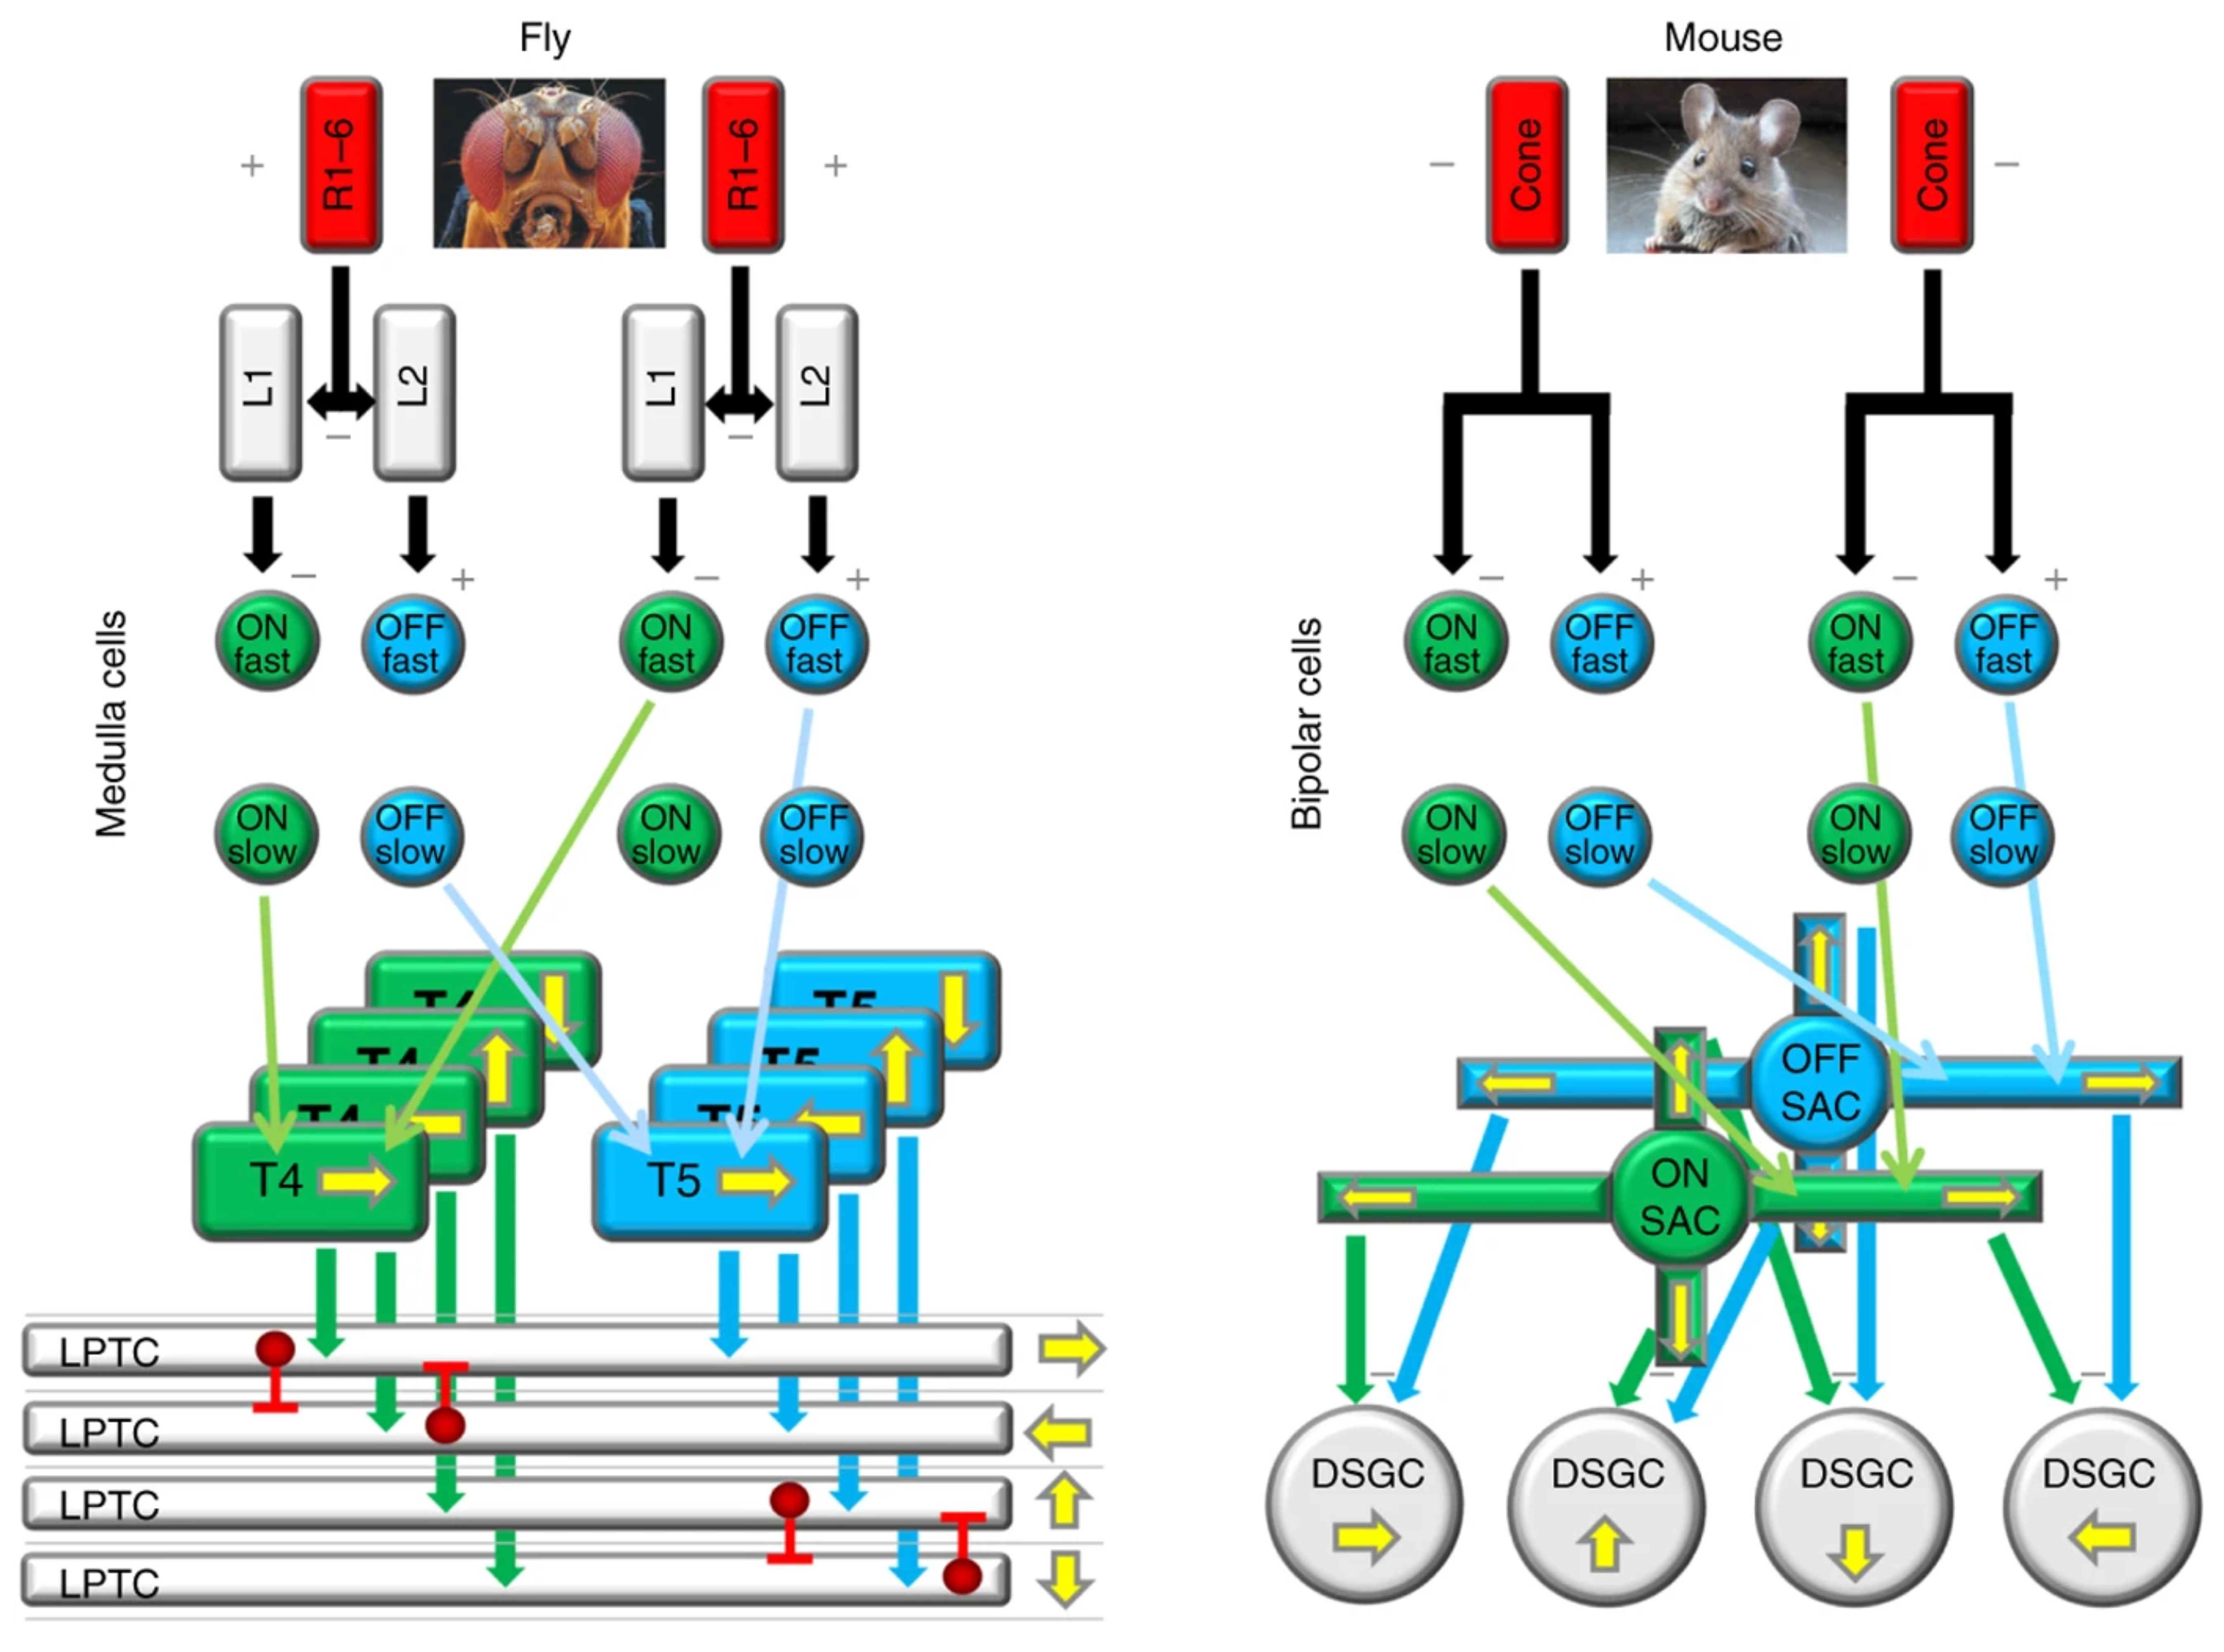
\includegraphics[scale=0.6]{fly_mouse_comparison}
\caption[Fly and mouse motion detection circuits] {Fly and mouse motion detection circuits: In the fly, the photoreceptors connect via sign-inverting synapses to the lamina monopolar cells L1 and L2, the entry to the ON and OFF pathway, respectively. The mouse retina lacks this additional layer of lamina cells and splits the signal directly between ON and OFF bipolar cells via two types of glutamate receptors. The T4 (ON) and T5 (OFF) neurons in the fly optic lobe and the ON and OFF SACs in the mouse retina are the first stages of direction-selective cells. Lobula plate tangential cells (LPTCs) in the fly and ON-OFF direction-selective ganglion cells (DSGCs) in the mouse integrate direction-selective information from these two pathways. (Used with permission from \cite{Borst2015})} 
\label{fig:flymouse}
\end{figure}

\section{Conclusion}
In the course of this work, I investigated neural computation in the \textit{Drosophila} motion vision pathway. Together with my co-authors, we showed that both the preferred direction enhancement and null direction suppression are implemented in all four subtypes of T4 and T5 cells. Already at the first stage of direction selectivity computation, this combined strategy ensures a high degree of direction selectivity. Additionally, we showed that the voltage-to-calcium transformations further enhance direction selectivity in the output signals of T4 cells in addition to the synaptic mechanisms at the dendrites. We built a model to transform voltage signals into calcium signals. The model was more complex for the direction-selective T4 cells compared to non-direction selective cells Mi1 and Tm3. Future work will focus on the comparison of voltage-gated calcium channels in these neurons which lead to different voltage to calcium transformations.



